\documentclass[../poliXuniversity_hospital_-USP-report.tex]{subfiles}
\graphicspath{ {images/}{../images/}{../../images/} }
\begin{document}
\clearpage
%================================ CONTROLE ========================
\section{Controle}

A placa de controle é a principal do robô. Ela foi idealizada, desde da primeira versão do robô hospitalar, para realizar o controle dos drivers dos motores, receber e enviar mensagens para os outros dispositivos embarcados e se comunicar diretamente com a Jetson \cite{jetson21}, um computador embarcado no robô feita para processar dados.

\subsection{Placa}

Como módulo principal, existem muitas minúcias que precisamos tomar ao projetá-las. A placa de controle, para segunda versão do robô hospitalar, com objetivo de evitar problemas e realizar testes, teve duas versões: um protótipo, que já foi finalizado, e uma versão oficial, ainda em desenvolvimento. 

%================================ CONTROLE PROTOTIPO ========================
\subsubsection{Protótipo}

O protótipo das placas foi refeito três vezes. Como se trata de uma placa fresada, pode ser refeita no próprio laboratório do professor orientador. O projeto da placa eletrônica, assim como o de todos os módulos, foi dividido em esquemático e Printed Circuit board (PCB) . 

\begin{figure}[!h]
\centering
    \caption{Protótipo placa de Controle - Esquemático principal }
    \centering % para centralizarmos a figura
    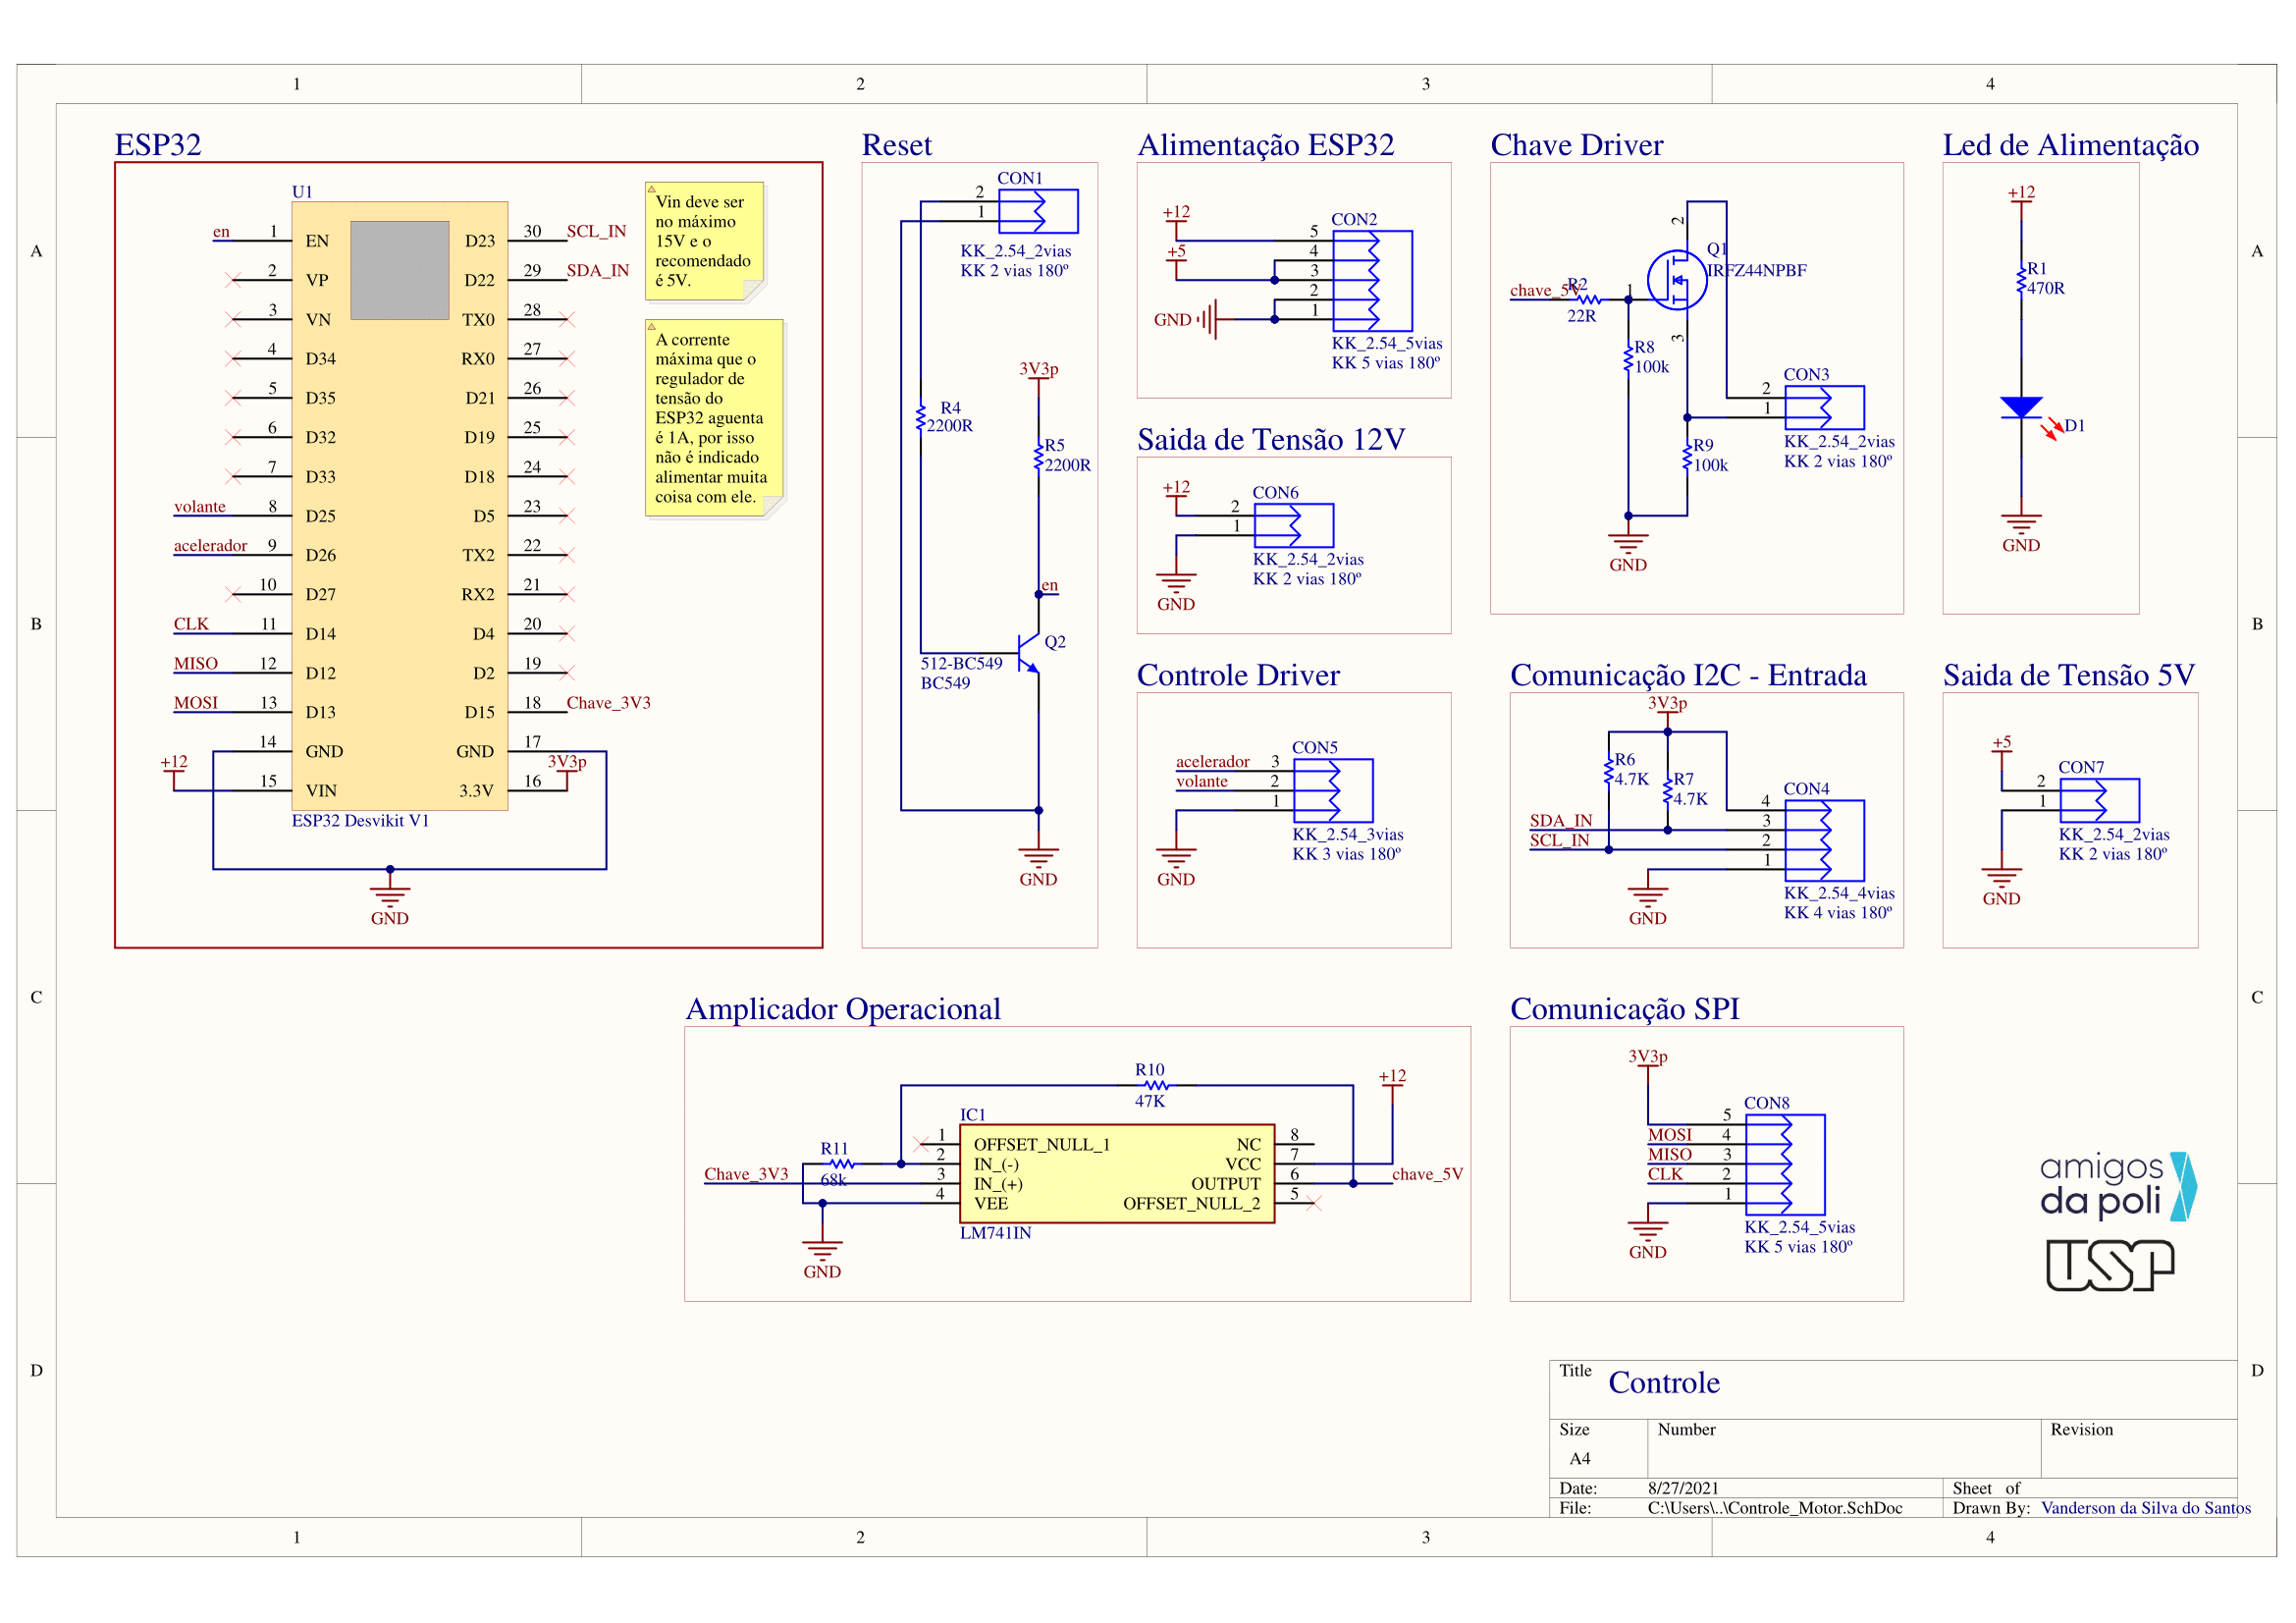
\includegraphics[width=17cm]{modulos/Controle_Motor-1.png}
    \caption*{Fonte: Elaborado pelo autor no software Altium Design\cite{altium21} }
    \label{Protótipo placa de ## - Esquemático principal}
\end{figure}

Para design do hardware do módulo de controle foi utilizado o CAD e software Altium Designer 21 \cite{altium21} a partir de uma licença estudantil. O projeto completo está disponibilizado em \cite{github_modulos} e todos os componentes usado nesse protótipo podem ser visto na tabela ~\ref{table:Componentes placa de Controle - Protótipo}.

\begin{table}[!h]
\caption{Componentes Utilizados na placa de Controle - Protótipo}
\centering
\begin{adjustbox}{width=\columnwidth,center}
\begin{tabular}{|c|c|c|c|c|}
\hline
Component                   & Description                                  & Designator             & Footprint                 & Quantity \\ \hline
4.7K                      & RES 4.7K OHM 1/4W 5\% CARBON FILM            & R6, R7                 & RES 4.7K 1/4W CARBON FILM & 2        \\ \hline
47K                       & RES 4.7K OHM 1/4W 5\% CARBON FILM            & R10                    & RES 4.7K 1/4W CARBON FILM & 1        \\ \hline
68k                       & RES 4.7K OHM 1/4W 5\% CARBON FILM            & R11                    & RES 4.7K 1/4W CARBON FILM & 1        \\ \hline
BC549                     & TRANS NPN 30V 0.1A TO-92                     & Q2                     & TO92                      & 1        \\ \hline
IRFZ44NPBF                & MOSFET (N-Channel)                           & Q1                     & TO254P483X1016X1994-3P    & 1        \\ \hline
KK\_2.54\_2vias           & Conector KK 2.54mm 2 vias                    & CON1, CON3, CON6, CON7 & KK\_2VIAS\_180º           & 4        \\ \hline
KK\_2.54\_3vias           & Conector KK 2.54mm 3 vias                    & CON5                   & KK\_3vias\_180º           & 1        \\ \hline
KK\_2.54\_4vias           & Conector KK 2.54mm 4 vias                    & CON4                   & KK\_4vias\_180°           & 1        \\ \hline
KK\_2.54\_5vias           & Conector KK 2.54mm 5 vias                    & CON2, CON8             & KK\_5vias\_180°           & 2        \\ \hline
LED 5MM RED               & LED 5MM RED                                  & D1                     & LED 5MM RED               & 1        \\ \hline
LM741IN                   & Integrated Circuit                           & IC1                    & DIP762W56P254L920H508Q8N  & 1        \\ \hline
microcontrolador          & microcontrolador com moculo bluethoth e wifi & U1                     & ESP32\_Desvikit\_v1       & 1        \\ \hline
RES 470R 1/4W CARBON FILM & RES 470R OHM 1/4W 5\% CARBON FILM            & R1, R2, R4, R5, R8, R9 & RES 470R 1/4W CARBON FILM & 6        \\ \hline
\end{tabular}
\end{adjustbox}
\centering
\caption*{Fonte: Elaborado pelo autor}
\label{table:Componentes placa de Controle - Protótipo}
\end{table}

\begin{figure}[h]
    \centering
    \begin{minipage}{0.5\textwidth}
        \centering
        \caption{Protótipo Controle - PCB 2D}
        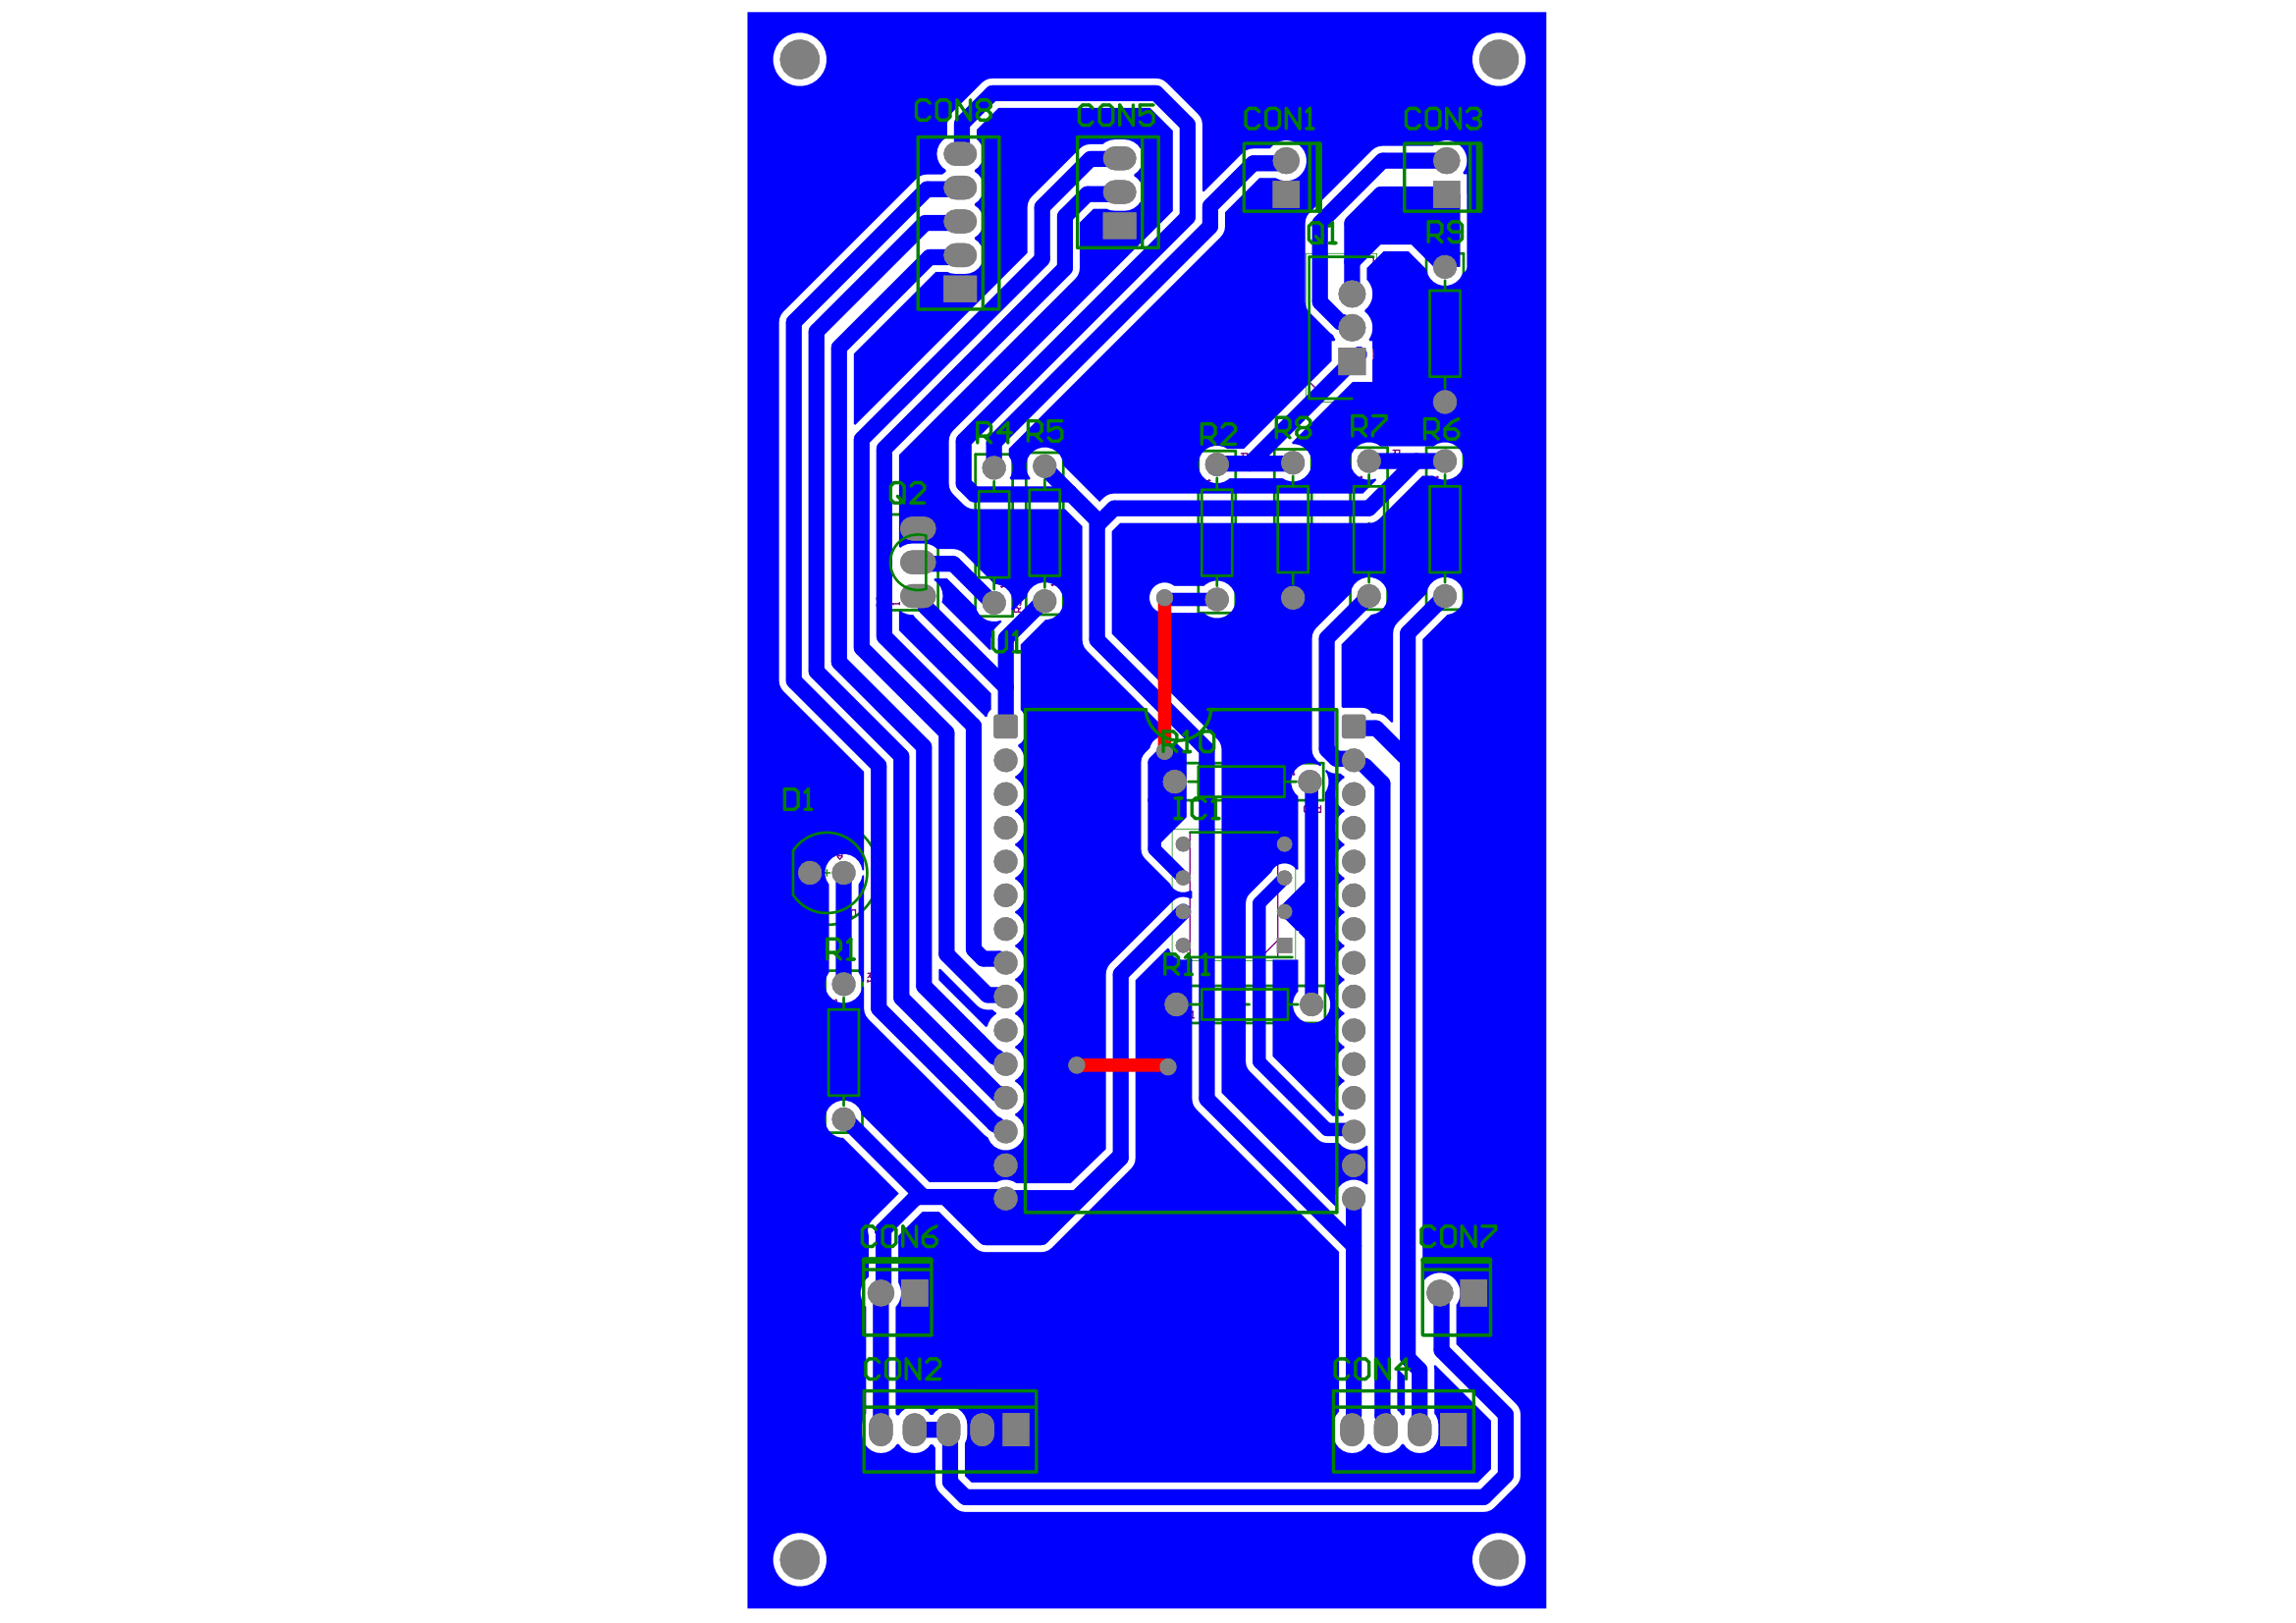
\includegraphics[width=1.03\textwidth]{modulos/Controle_Motor-2.png} 
        \label{fig:figura1minipg}
    \end{minipage}\hfill
    \begin{minipage}{0.5\textwidth}
        \centering
        \caption{Protótipo Controle - PCB 3D }
        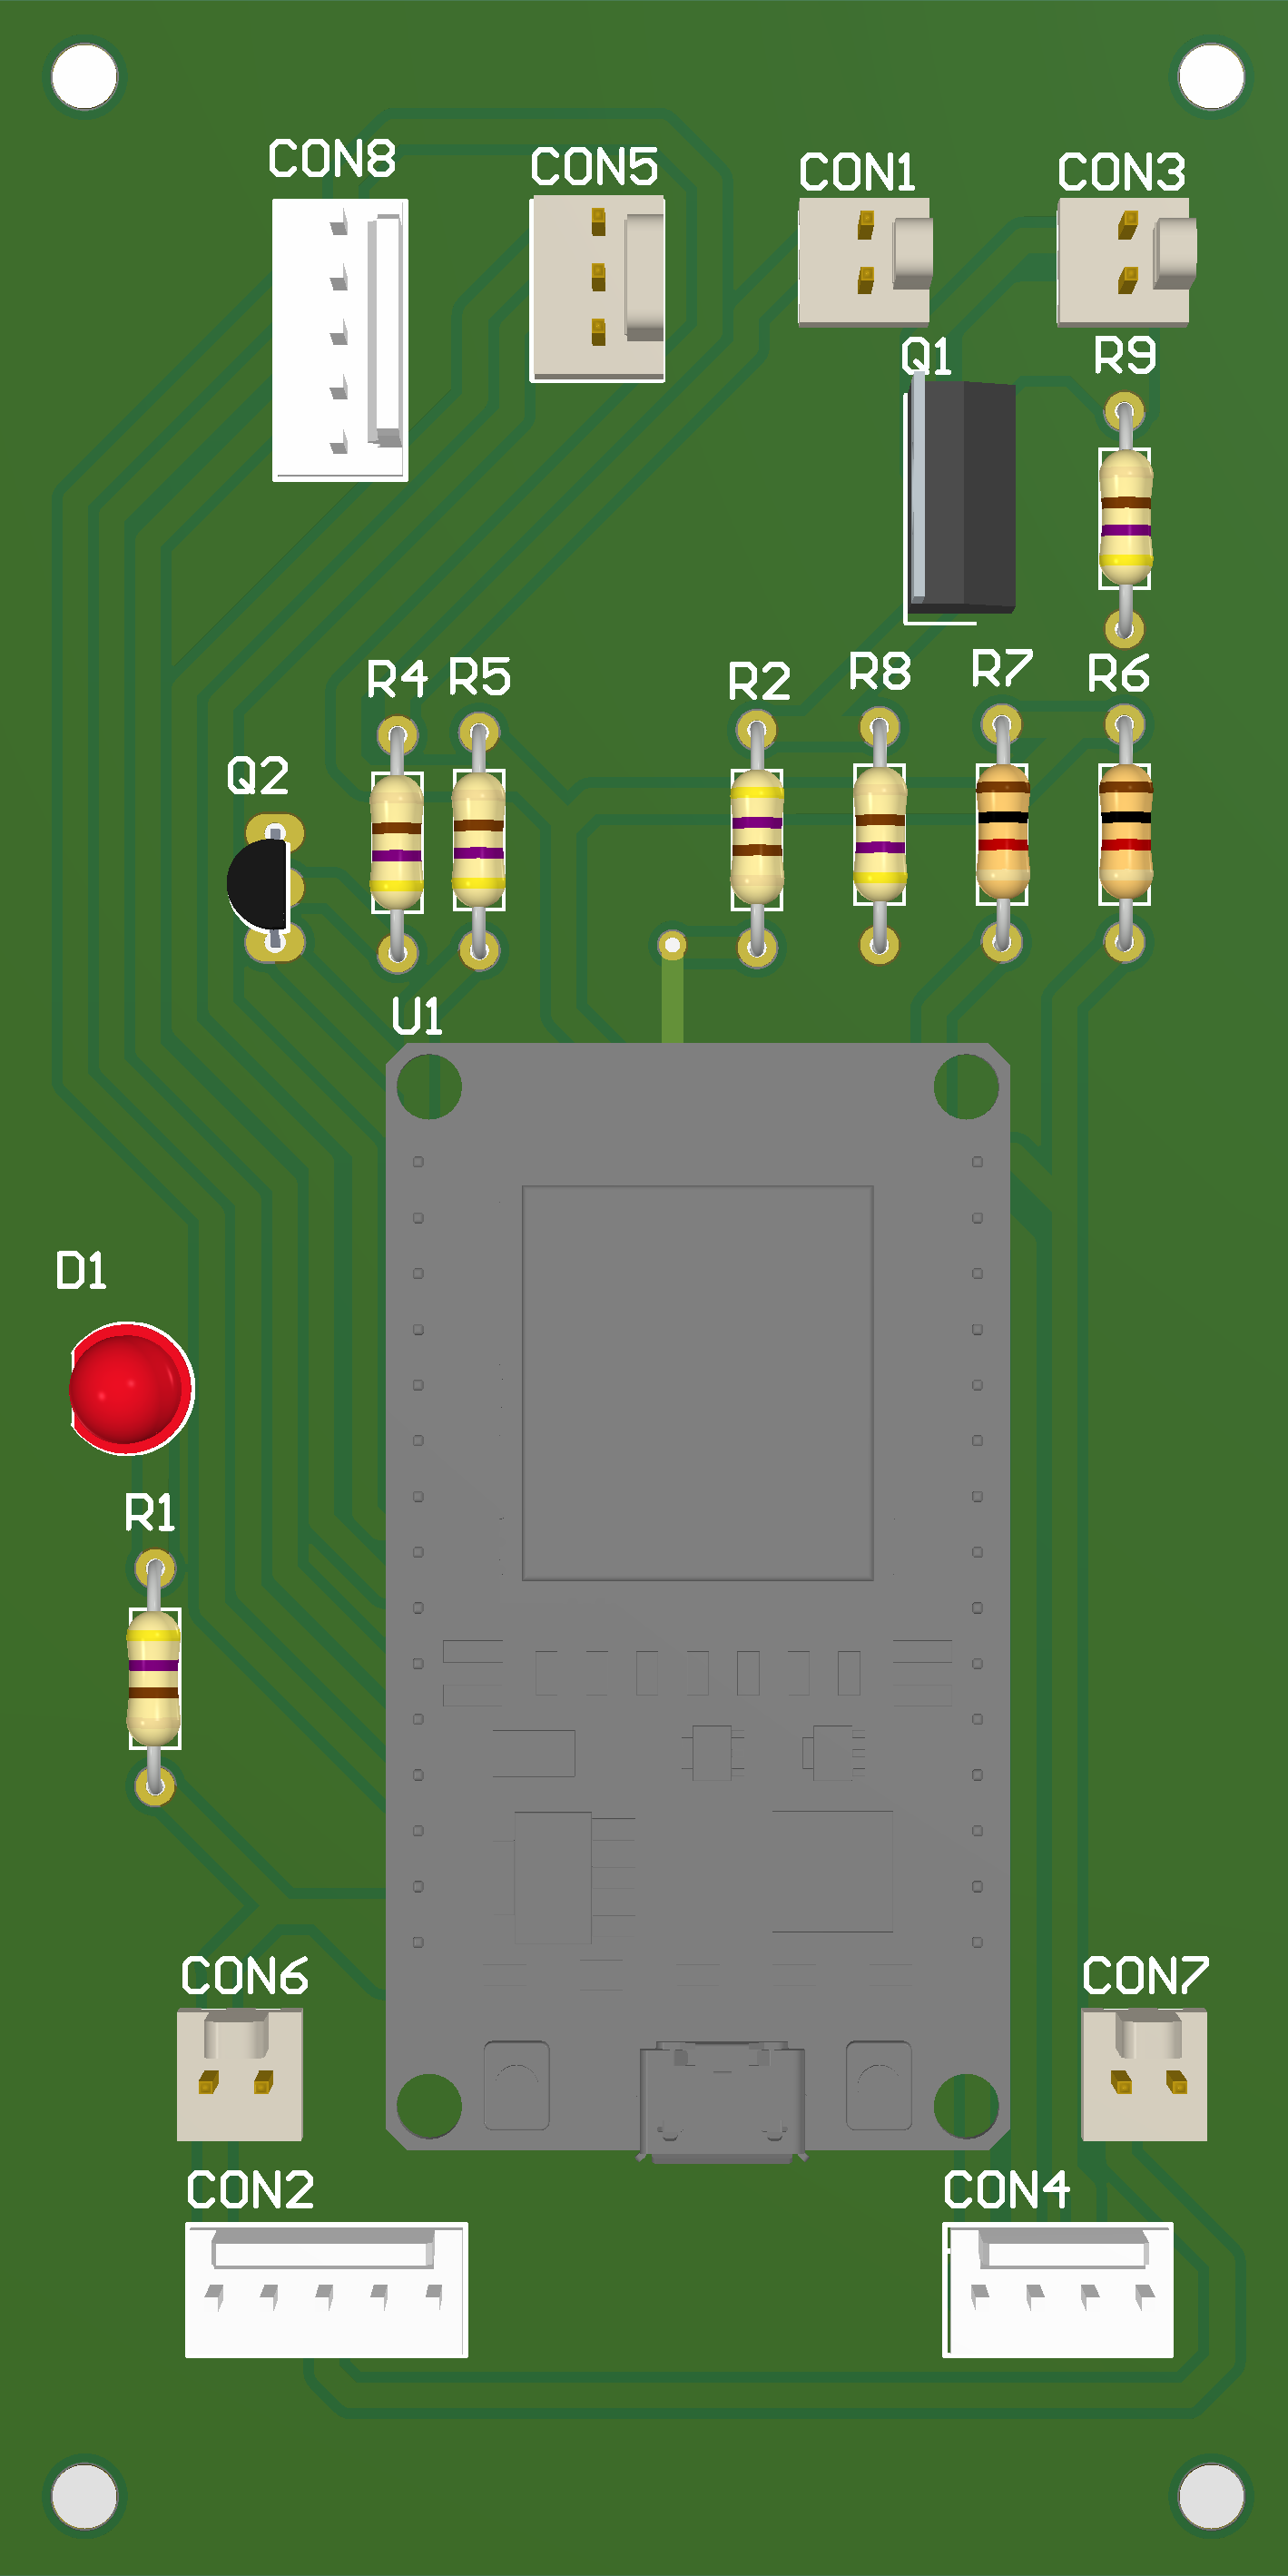
\includegraphics[width=0.4\textwidth]{modulos/Controle_Motor.png} 
        \label{fig:figura1minipg}
    \end{minipage}\hfill
    
    \caption*{Fonte: Elaborado pelo autor no software Altium Design\cite{altium21} }
    \label{fig:2d3dcontrolepro}
\end{figure}

Dentre os componentes usados, destaca-se o transistor mosfet  IRFZ44NPBF \cite{IRFZ44NPBF_datasheet}, utilizado no circuito da chave do driver e o amplificador operacional LM741 \cite{LM741_datasheet}, usado para envío de pequenos sinais no circuito para o driver.

\begin{comment}
\begin{figure}[h]
    \centering
    \begin{minipage}{0.5\textwidth}
        \centering
        \caption{Protótipo Controle - Trilhas}
        \includegraphics[width=0.8\textwidth]{example-image-a} 
        \label{fig:figura1minipg}
    \end{minipage}\hfill
    \begin{minipage}{0.5\textwidth}
        \centering
        \caption{Protótipo Controle - Completa }
        \includegraphics[width=0.8\textwidth]{example-image-a} 
        \label{fig:figura1minipg}
    \end{minipage}\hfill
    
    \caption*{Fonte: Elaborado pelo autor }
    \label{fig:2d3dcontroleproreal}
\end{figure}
\end{comment}
%================================ CONTROLE OFICIAL ========================
\clearpage
\subsubsection{Oficial}

A placa oficial de controle ainda não foi fabricada. Por se tratar de uma placa mais profissional, ela será mandada para ser feita para uma empresa privada ainda não escolhida, não na própria Universidade São Paulo. Assim como o protótipo, o projeto como um todo foi dividido em um esquemático e uma PCB.

\begin{figure}[h]
\centering
    \caption{Placa de Controle - Esquemático principal }
    \centering % para centralizarmos a figura
    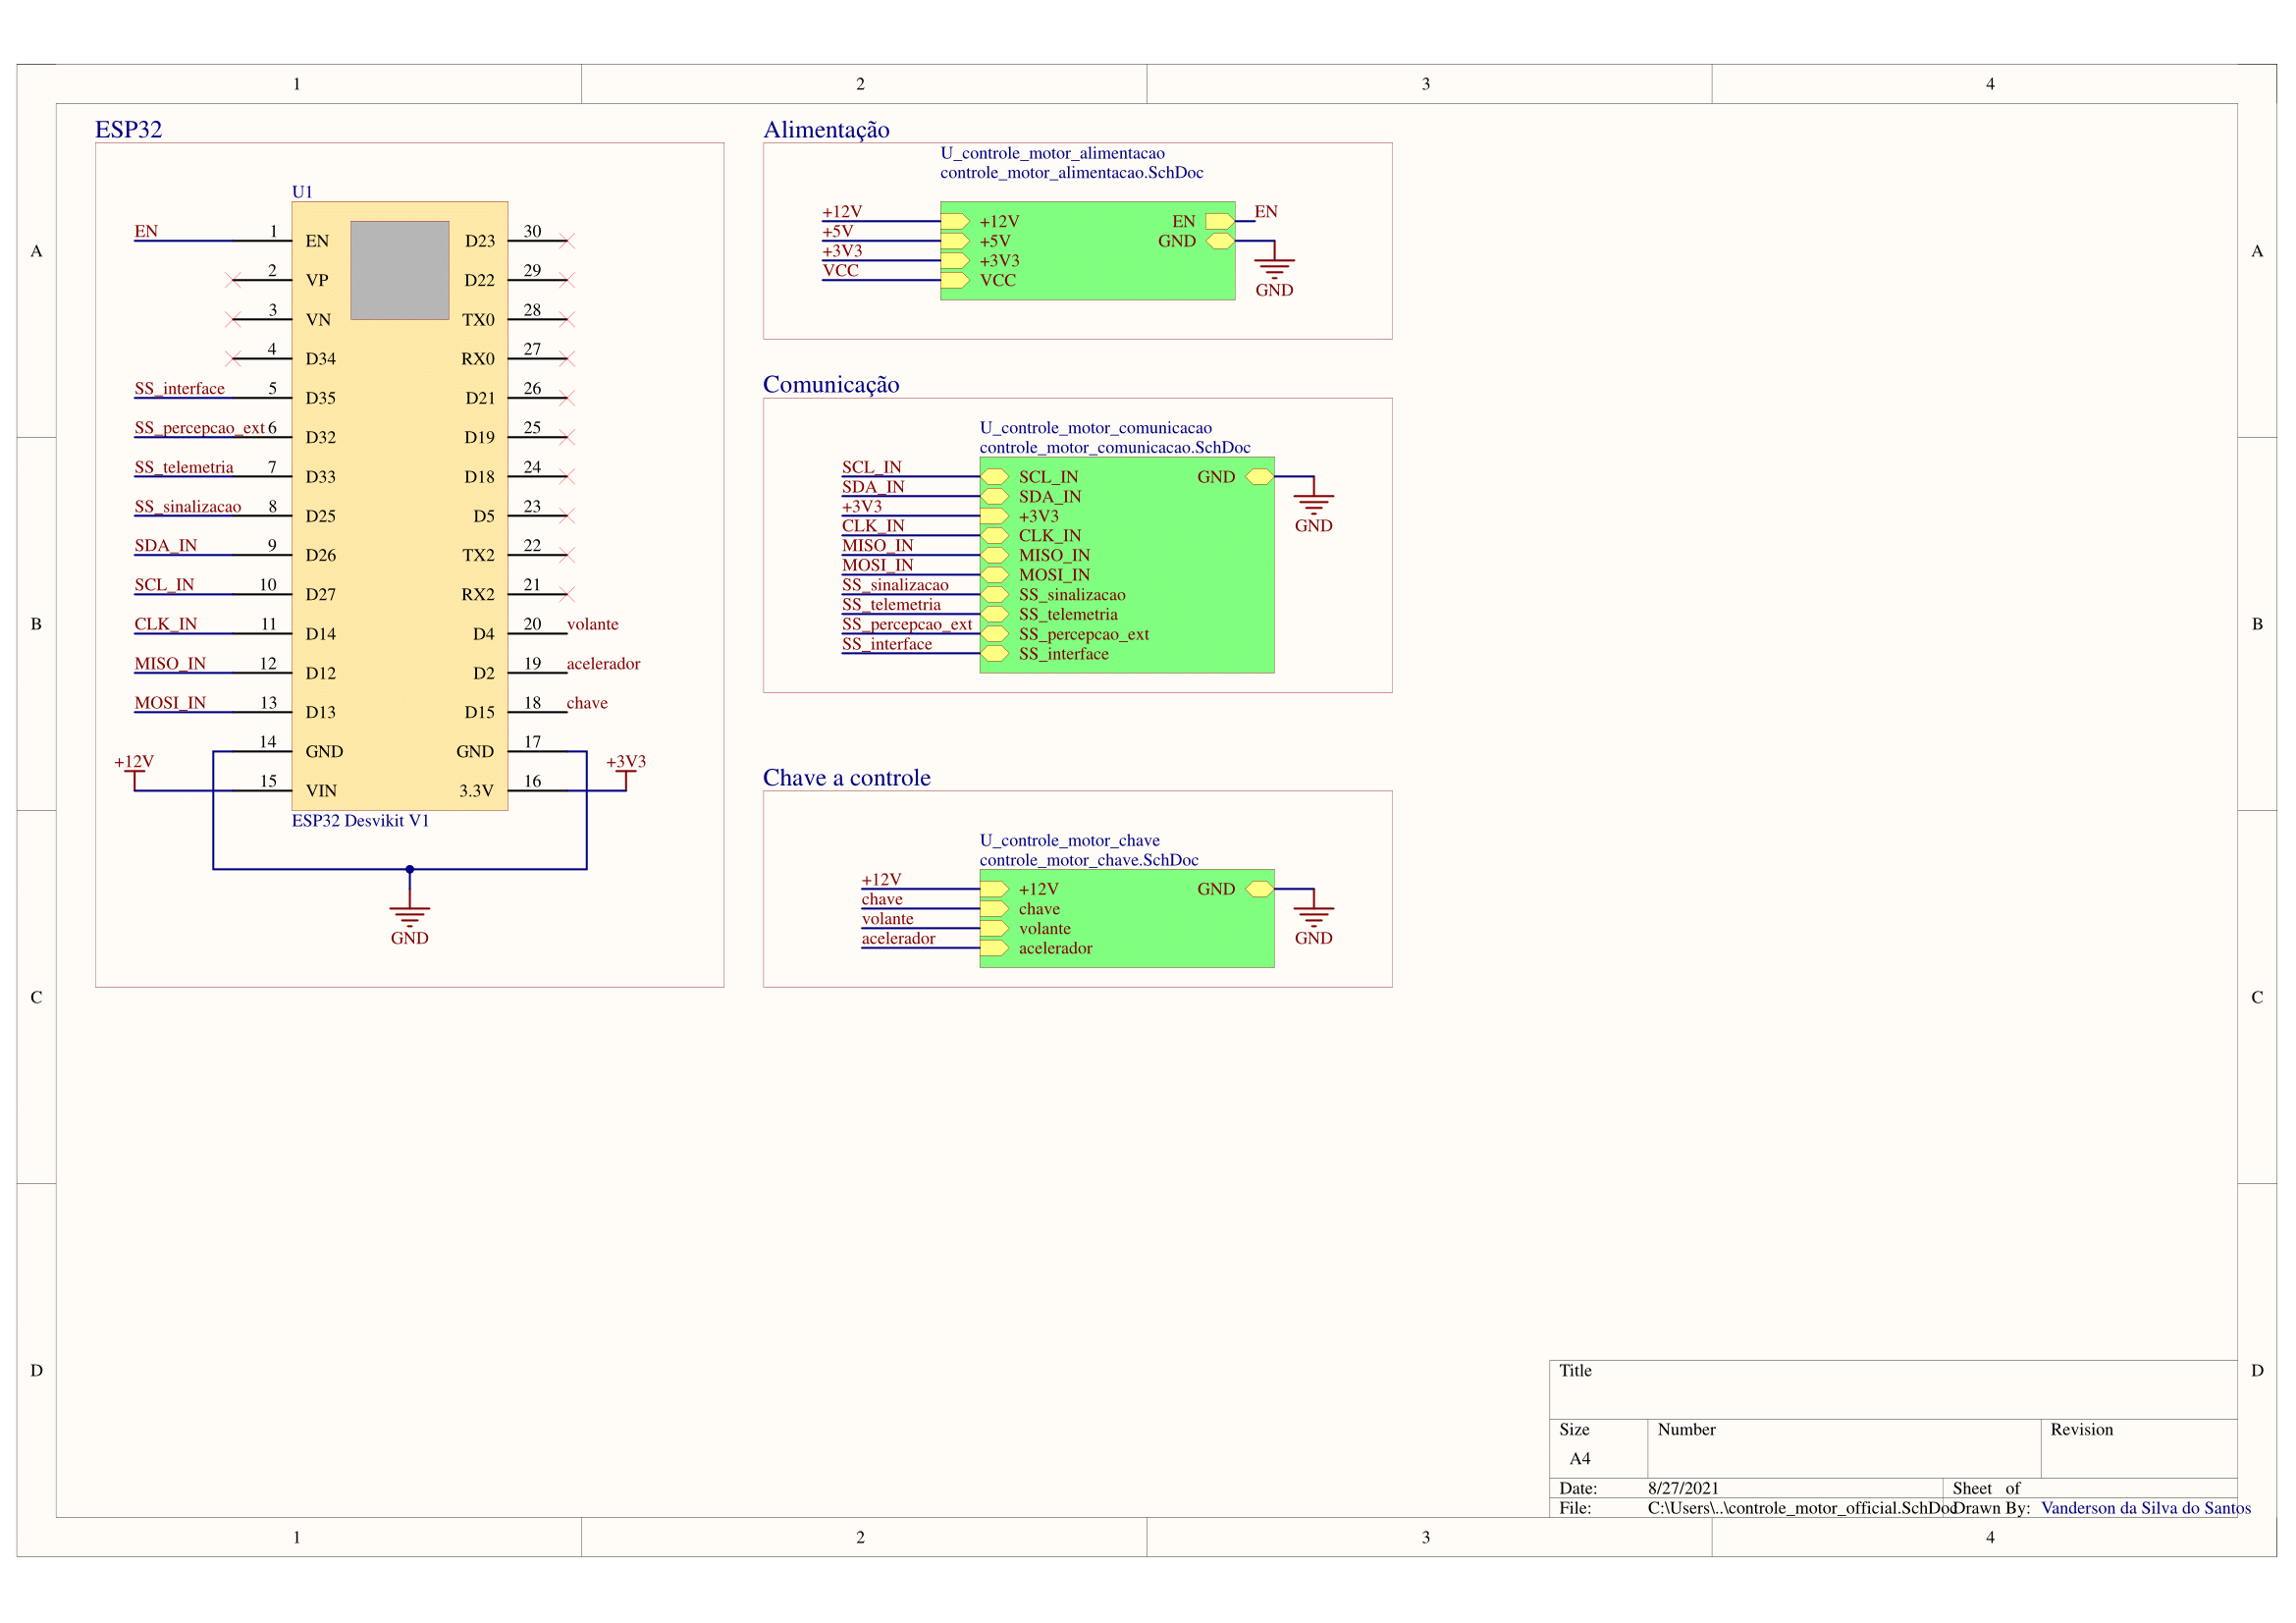
\includegraphics[width=15cm]{modulos/controle_motor_official-1.png}
    \caption*{Fonte: Elaborado pelo autor no software Altium Design\cite{altium21} }
    \label{Placa de Controle - Esquemático principal}
\end{figure}

Para design do hardware do módulo de controle foi utilizado o CAD e software Altium Designer 21 \cite{altium21} a partir de uma licença estudantil. O projeto completo está disponibilizado em \cite{github_modulos} e todos os componentes usado nessa versão oficial podem ser visto na tabela ~\ref{Componentes Utilizados na placa de Controle}.

\begin{table}[h]
\caption{Componentes Utilizados na placa de Controle}
\centering
\begin{adjustbox}{width=\columnwidth,center}
\begin{tabular}{|c|c|c|c|c|}
\hline
Component        & Description                                    & Designator                 & Footprint                & Quantity \\ \hline
KK\_2.54\_5vias  & Conector KK 2.54mm 5   vias                    & CON1, CON7, CON10,   CON11 & KK\_5vias\_180°          & 4        \\ \hline
KK\_2.54\_4vias  & Conector KK 2.54mm 4   vias                    & CON2                       & KK\_4vias\_180°          & 1        \\ \hline
KK\_2.54\_2vias  & Conector KK 2.54mm 2   vias                    & CON3, CON5, CON6,   CON8   & KK\_2VIAS\_180º          & 4        \\ \hline
KK\_2.54\_6vias  & Conector KK 2.54mm 6   vias                    & CON4                       & KK\_6vias\_180°          & 1        \\ \hline
KK\_2.54\_3vias  & Conector KK 2.54mm 3   vias                    & CON9                       & KK\_3vias\_180º          & 1        \\ \hline
LED 3MM RED      & LED 3MM RED                                    & D1                         & LED RED                  & 1        \\ \hline
LM741IN          & Integrated Circuit                             & IC1                        & DIP762W50P254L712H450Q6N & 1        \\ \hline
Trans BC817      & Transistor BJT NPN   BC817-25-7-F              & Q1                         & SOT96P240X110-3N         & 1        \\ \hline
IRFZ44NPBF       & MOSFET (N-Channel)                             & Q2                         & TO254P483X1016X1994-3P   & 1        \\ \hline
4k7              & RES 1206 5\%                                   & R1, R2                     & RESC3216X60N             & 2        \\ \hline
680R             & Resistor                                       & R3                         & RESC3216X60N             & 1        \\ \hline
2k2              & Resistor                                       & R4, R5                     & RESC3216X60N             & 2        \\ \hline
47K              & RES 1206 5\%                                   & R6                         & RESC3216X60N             & 1        \\ \hline
68k              & 0805                                           & R7                         & RESISTOR 0805            & 1        \\ \hline
22R              & RES 1206 5\%                                   & R8                         & RESC3216X60N             & 1        \\ \hline
100k             & RES 1206 5\%                                   & R9, R10                    & RESC3216X60N             & 2        \\ \hline
microcontrolador & microcontrolador com   moculo bluethoth e wifi & U1                         & ESP32\_Desvikit\_v1      & 1        \\ \hline

\end{tabular}
\end{adjustbox}
\centering
\caption*{Fonte: Elaborado pelo autor}
\label{Componentes Utilizados na placa de Controle}
\end{table}

Em relação ao protótipo, pouco mudou da lógica por trás do circuito, a principal diferença é que o modelo oficial utiliza todos componentes com encapsulamiento SMD \cite{SMD_def}. Além disso, foi adicionado o protocolo de comunicação SPI também, como já foi comentado no início do capítulo.

A placa de circuito impresso ainda está em desenvolvimento.

%================================ CONTROLE FIRMWARE ========================
\begin{comment}
\subsection{Firmware}
\end{comment}

\subsection{Driver do Motor}

O motor do robô hospitalar é trifásico. A construção de uma ESC para controle adequado e preciso do motor é um trabalho muito minucioso e preciso. Por conta disso, como decisão de projeto, os integrantes do grupo preferiram comprar um driver que a conseguisse realizar o controle de segurança. A imagem do driver pode ser vista na figura ~\ref{fig:Driver de Controle do Motor}.

\begin{figure}[h]
\centering
    \caption{Driver de Controle do Motor}
    \centering % para centralizarmos a figura
    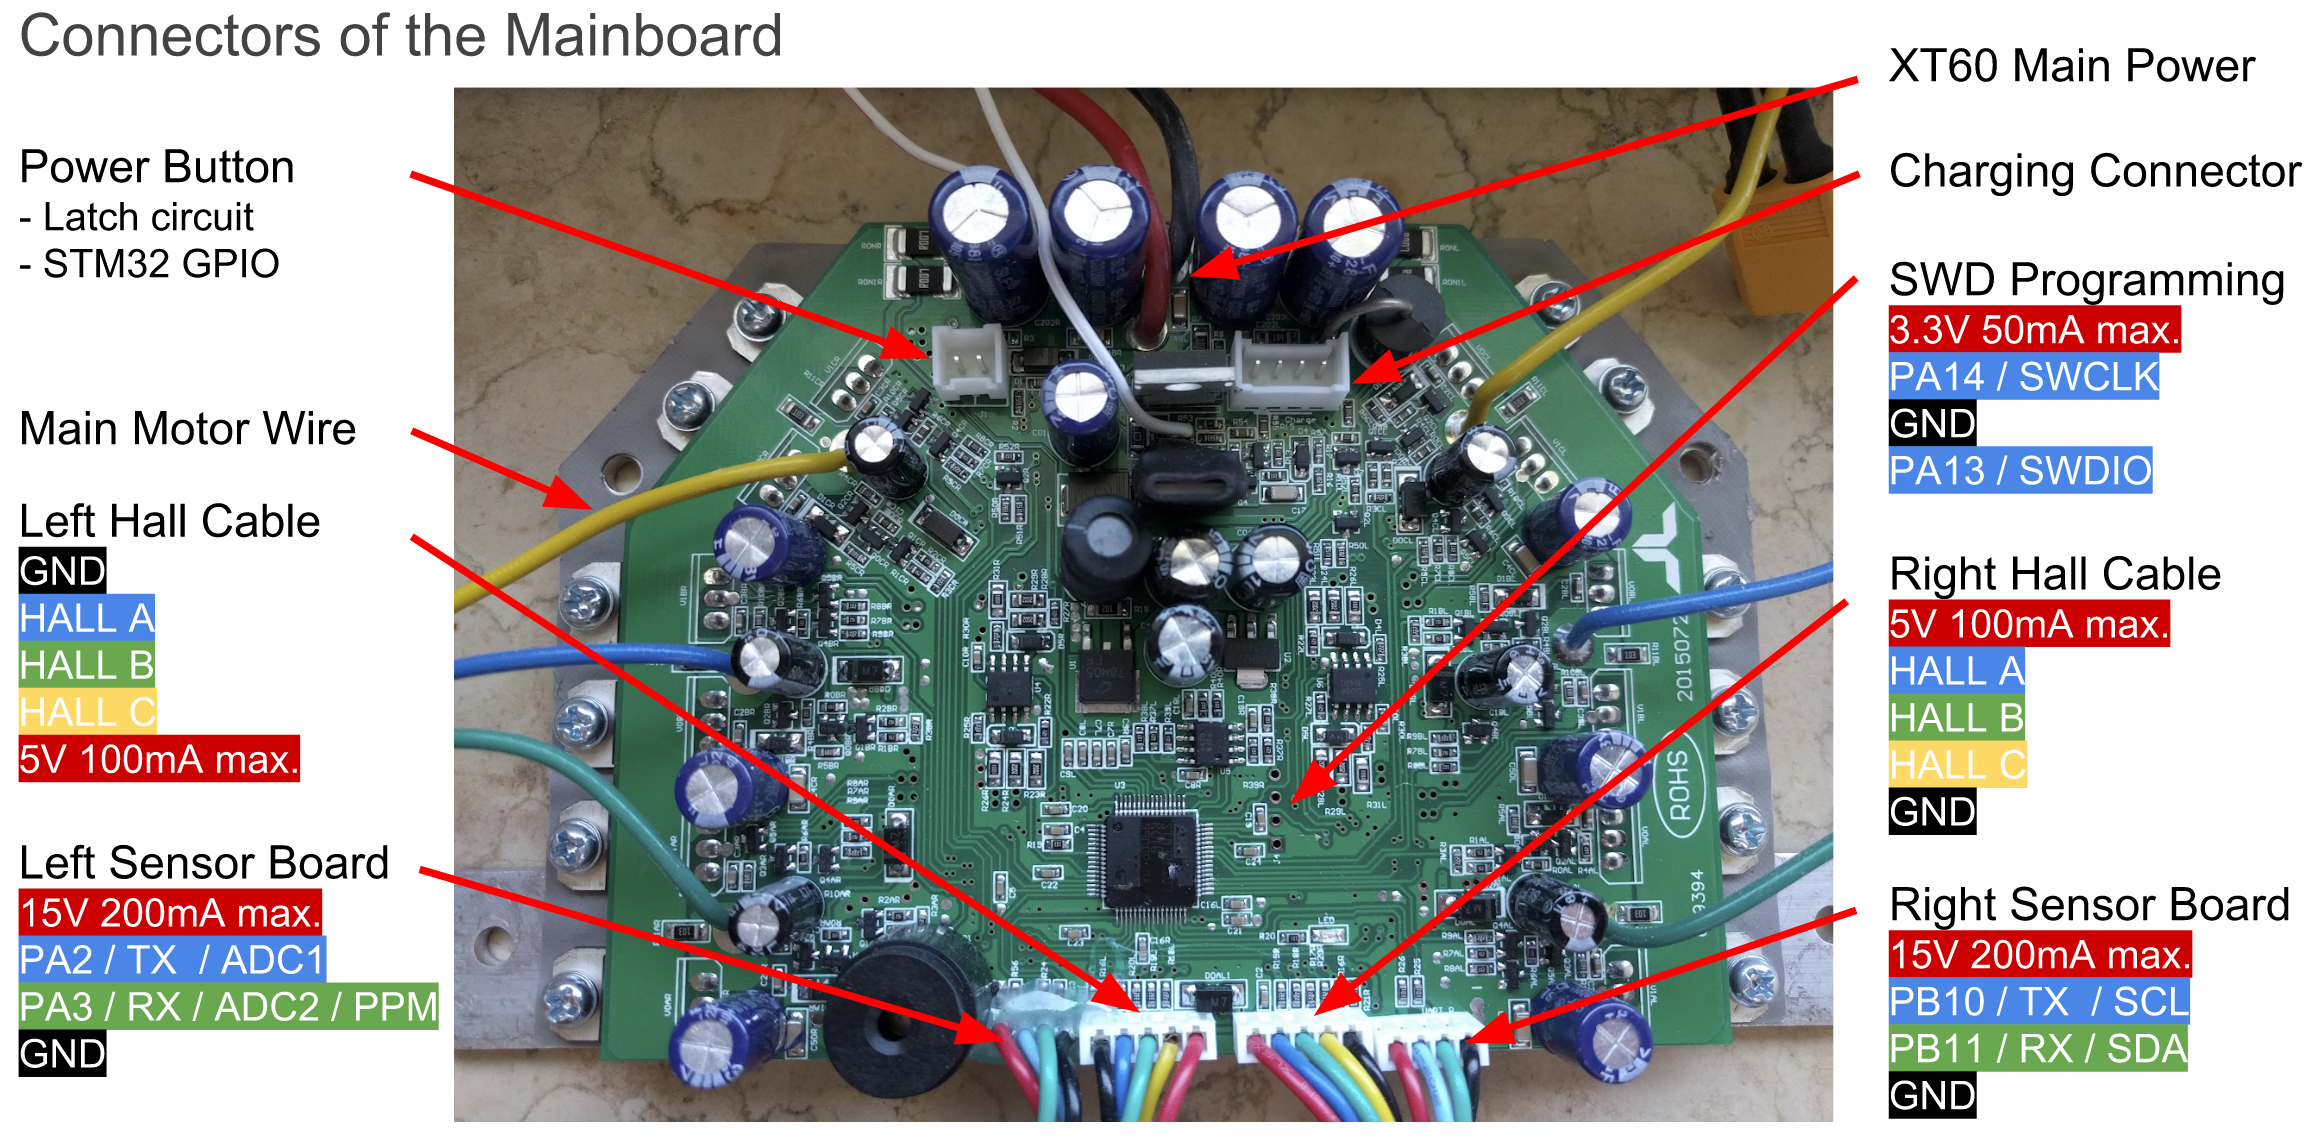
\includegraphics[width=15cm]{driver_motor.png}
    \caption*{Fonte: imagem retirada de \cite{drivermotor21}}
    \label{fig:Driver de Controle do Motor}
\end{figure}

Entretanto, ainda há necessidade de controlar adequadamente esse driver, o qual é a função da placa de controle.

\end{document}
